\paragraph{Phạm vi chạy thực tế} Dữ liệu có 180519 dòng; thí nghiệm dùng 5999 dòng: train 4823, test 1176. Số nhóm tương ứng là 1690 và 423.

\begin{table}[!htbp]\centering\resizebox{\textwidth}{!}{\begin{tabular}{lrrrrrr}
\hline
Model & Train F1 & CV F1 & Acc & Prec & Recall & F1 \\
\hline
baseline\_tree\_A & 0.999 & 0.669 & 0.653 & 0.699 & 0.623 & 0.659 \\
dummy\_A & 0.694 & 0.694 & 0.537 & 0.537 & 1.000 & 0.699 \\
knn\_A & 0.999 & 0.667 & 0.673 & 0.723 & 0.636 & 0.677 \\
tree\_A & 0.765 & 0.674 & 0.646 & 0.673 & 0.665 & 0.669 \\
knn\_B & 1.000 & 0.671 & 0.686 & 0.729 & 0.661 & 0.694 \\
tree\_B & 0.714 & 0.706 & 0.733 & 0.853 & 0.608 & 0.710 \\
\hline
\end{tabular}}\caption{So sánh metric theo dòng của các cấu hình trên CV và tập kiểm tra lịch sử.}\label{tab:model-comparison}\end{table}

Mô hình chọn trước đánh giá test: tree\_B; CV F1=0.7058, cao nhất trong sáu cấu hình được báo cáo. Việc chọn dựa trên CV trước khi đánh giá holdout. Accuracy=0.7330, Precision=0.8533, Recall=0.6076, F1=0.7098. ROC-AUC=0.7756, PR-AUC=0.7889.

Ma trận nhầm lẫn: TN=478, FP=66, FN=248, TP=384. Không coi recall cao của Dummy (dự đoán tất cả trễ) là bằng chứng mô hình hữu ích.

knn: B−A CV F1=0.0046; test F1=0.0170.

tree: B−A CV F1=0.0316; test F1=0.0410.

Cây mặc định có train F1=0.9994, CV F1=0.6691; chênh lệch lớn gợi ý overfitting. Mô hình chọn có chênh lệch train--CV=0.0079. Một split chưa cho phép kết luận tổng quát.

First Class: 203 dòng, 193 dương, FN=0, FP=10. FNR=0.0000, FPR=1.0000.

Same Day: 71 dòng, 27 dương, FN=0, FP=0. FNR=0.0000, FPR=0.0000.

Second Class: 198 dòng, 158 dương, FN=0, FP=40. FNR=0.0000, FPR=1.0000.

Standard Class: 704 dòng, 254 dương, FN=248, FP=16. FNR=0.9764, FPR=0.0356.

Lỗi tập trung cần được điều tra bằng dữ liệu vận hành; đây là bằng chứng mô tả, không là nguyên nhân đã xác minh. Không điều chỉnh mô hình dựa trên những quan sát test này.

\begin{figure}[!htbp]\centering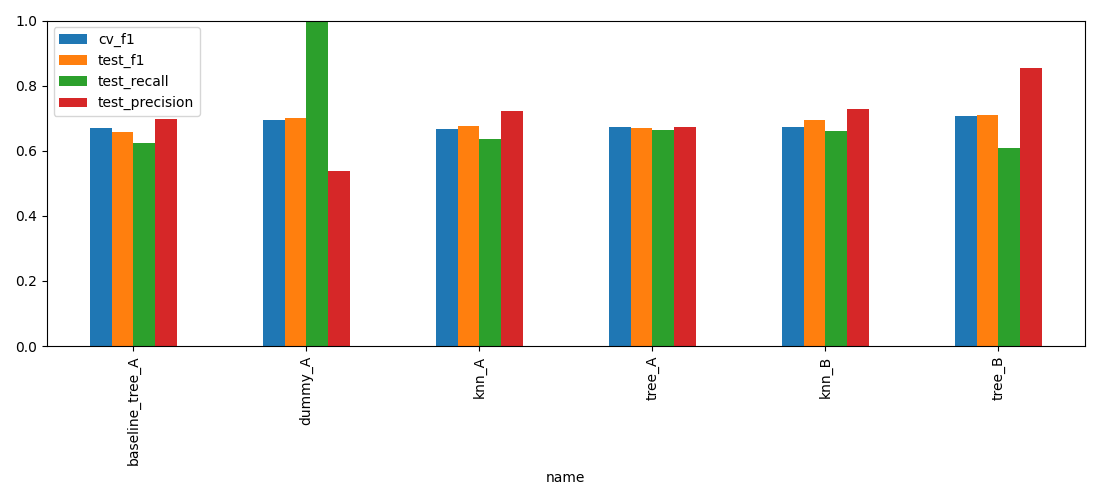
\includegraphics[width=.90\textwidth,height=.42\textheight,keepaspectratio]{../results/figures/comparison.png}\caption{So sánh các cấu hình mô hình theo CV và tập kiểm tra.}\label{fig:comparison}\end{figure}

\begin{figure}[!htbp]\centering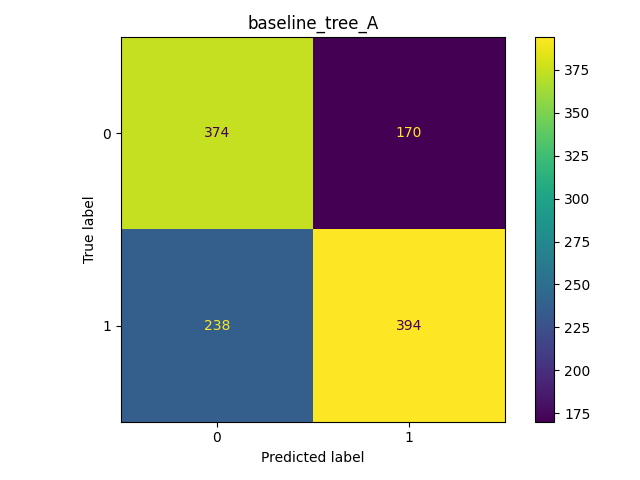
\includegraphics[width=.90\textwidth,height=.42\textheight,keepaspectratio]{../results/figures/baseline_tree_A_confusion.png}\caption{Ma trận nhầm lẫn theo dòng: Baseline cây quyết định với luồng A.}\label{fig:confusion-baseline}\end{figure}

\begin{figure}[!htbp]\centering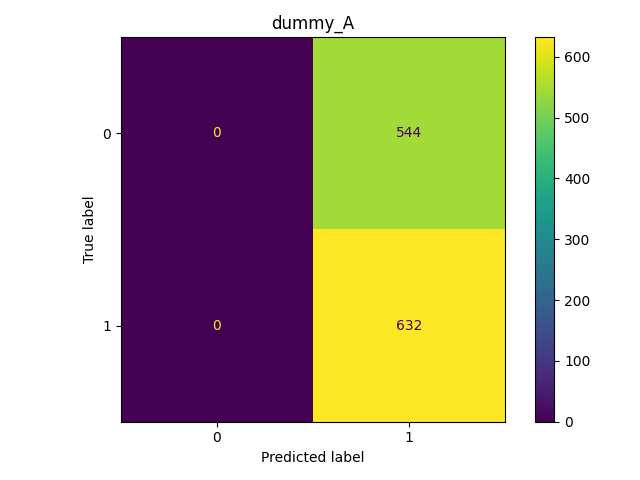
\includegraphics[width=.90\textwidth,height=.42\textheight,keepaspectratio]{../results/figures/dummy_A_confusion.png}\caption{Ma trận nhầm lẫn theo dòng: Baseline Dummy với luồng A.}\label{fig:confusion-dummy}\end{figure}

\begin{figure}[!htbp]\centering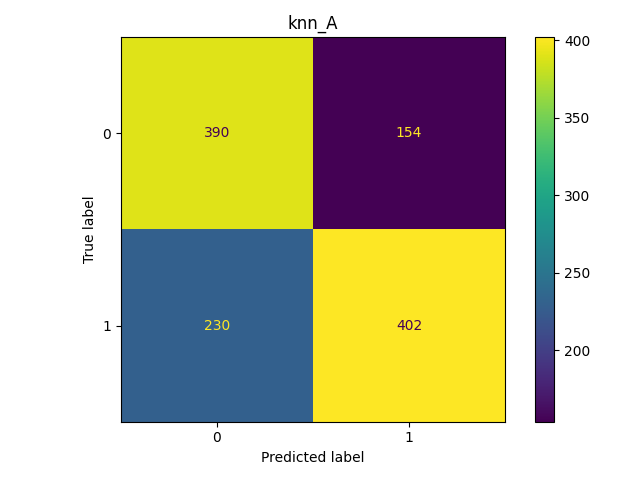
\includegraphics[width=.90\textwidth,height=.42\textheight,keepaspectratio]{../results/figures/knn_A_confusion.png}\caption{Ma trận nhầm lẫn theo dòng: K-NN với luồng A.}\label{fig:confusion-knn-a}\end{figure}

\begin{figure}[!htbp]\centering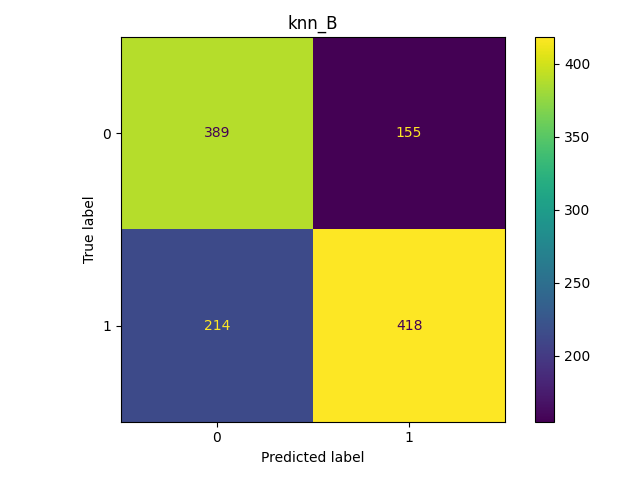
\includegraphics[width=.90\textwidth,height=.42\textheight,keepaspectratio]{../results/figures/knn_B_confusion.png}\caption{Ma trận nhầm lẫn theo dòng: K-NN với luồng B.}\label{fig:confusion-knn-b}\end{figure}

\begin{figure}[!htbp]\centering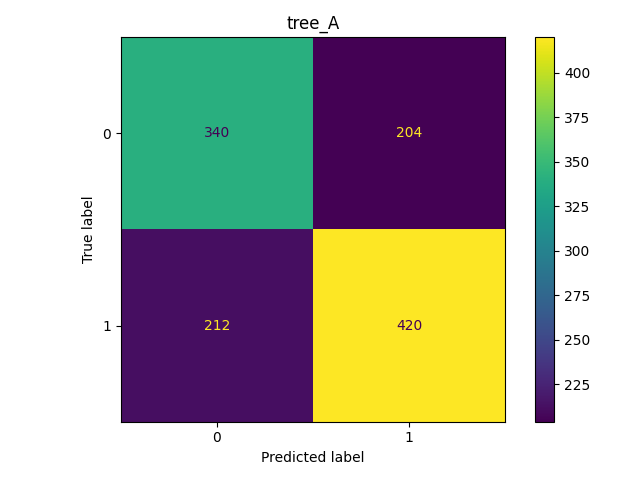
\includegraphics[width=.90\textwidth,height=.42\textheight,keepaspectratio]{../results/figures/tree_A_confusion.png}\caption{Ma trận nhầm lẫn theo dòng: Cây quyết định với luồng A.}\label{fig:confusion-tree-a}\end{figure}

\begin{figure}[!htbp]\centering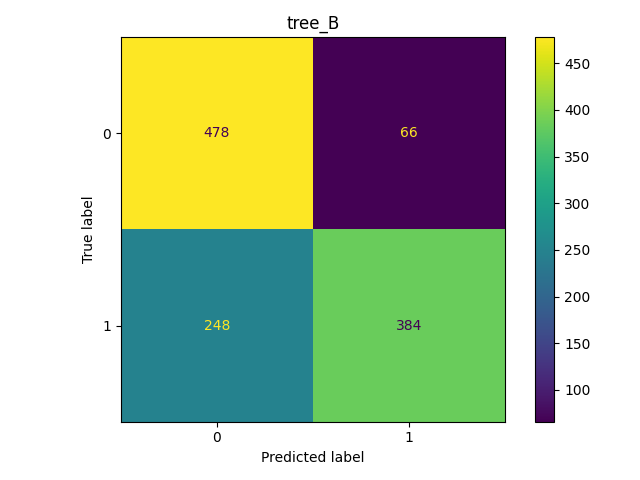
\includegraphics[width=.90\textwidth,height=.42\textheight,keepaspectratio]{../results/figures/tree_B_confusion.png}\caption{Ma trận nhầm lẫn theo dòng: Cây quyết định với luồng B. Mô hình được chọn bằng CV.}\label{fig:confusion-tree-b}\label{fig:selected-confusion}\end{figure}

\begin{figure}[!htbp]\centering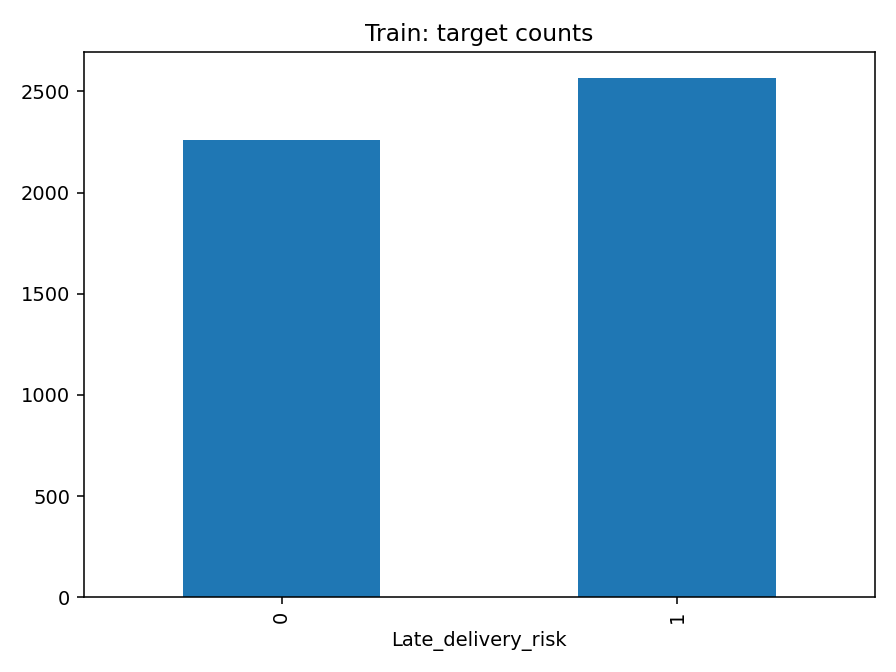
\includegraphics[width=.90\textwidth,height=.42\textheight,keepaspectratio]{../results/figures/01_classes.png}\caption{Phân bố nhãn trên tập huấn luyện.}\label{fig:eda-classes}\end{figure}

\begin{figure}[!htbp]\centering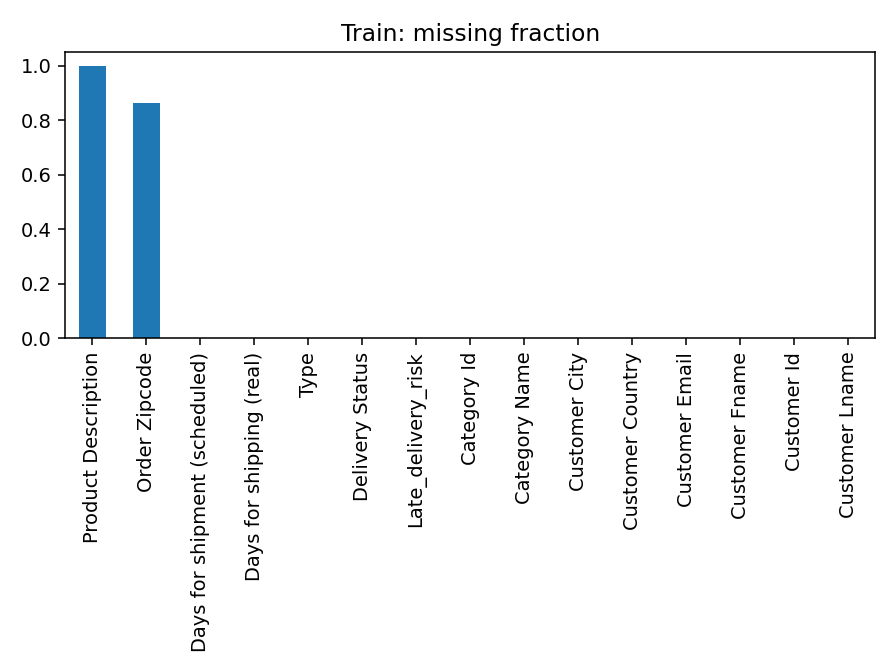
\includegraphics[width=.90\textwidth,height=.42\textheight,keepaspectratio]{../results/figures/02_missing.png}\caption{Tỷ lệ giá trị thiếu của các đặc trưng được khảo sát trên tập huấn luyện.}\label{fig:eda-missing}\end{figure}

\begin{figure}[!htbp]\centering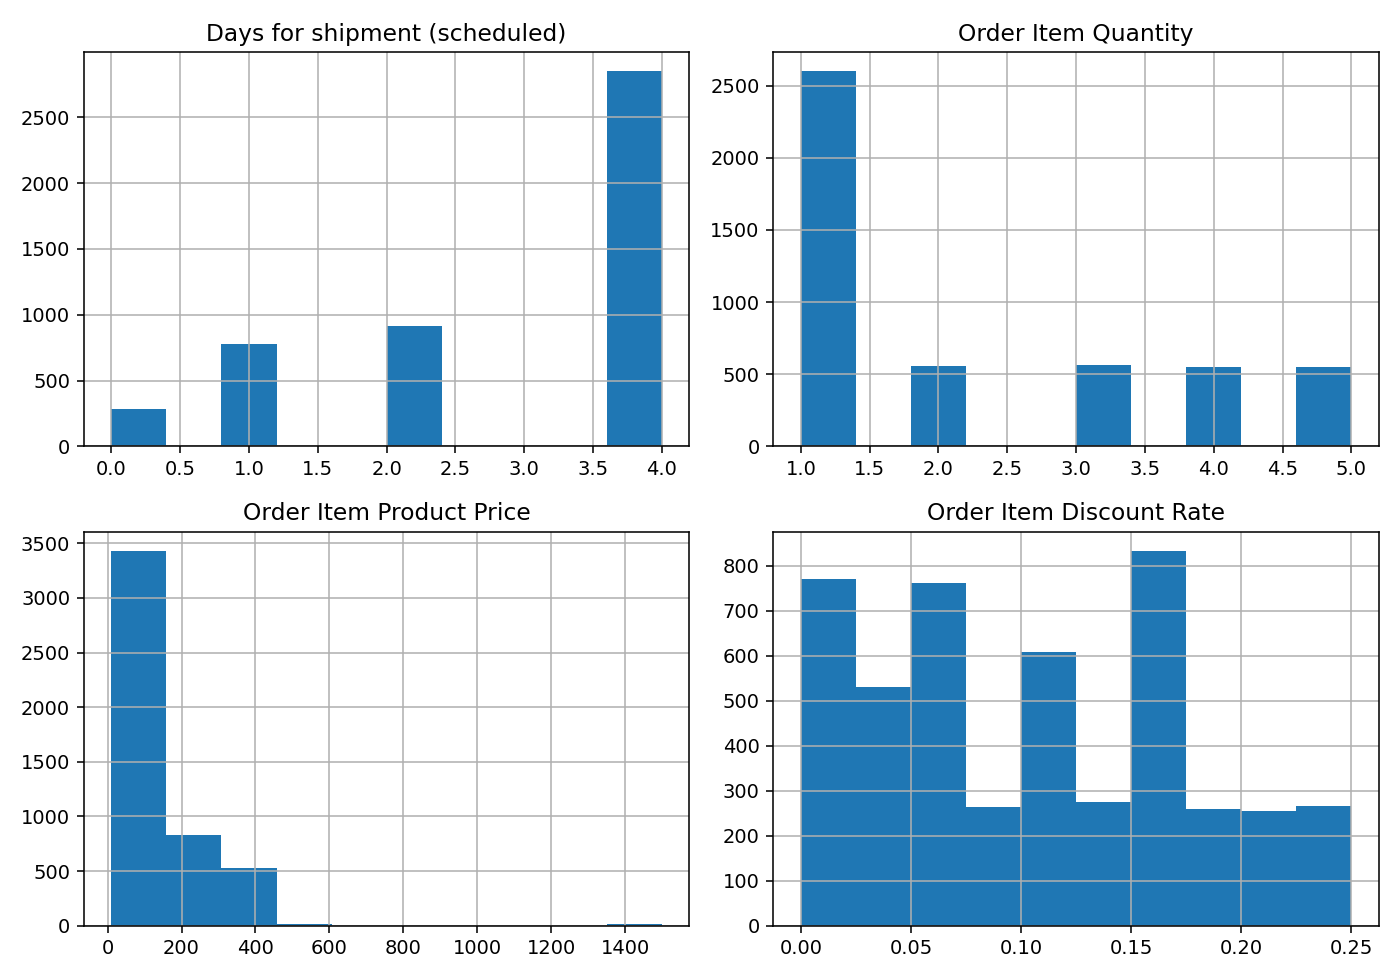
\includegraphics[width=.90\textwidth,height=.42\textheight,keepaspectratio]{../results/figures/03_numeric_hist.png}\caption{Phân bố các đặc trưng số trên tập huấn luyện.}\label{fig:eda-numeric}\end{figure}

\begin{figure}[!htbp]\centering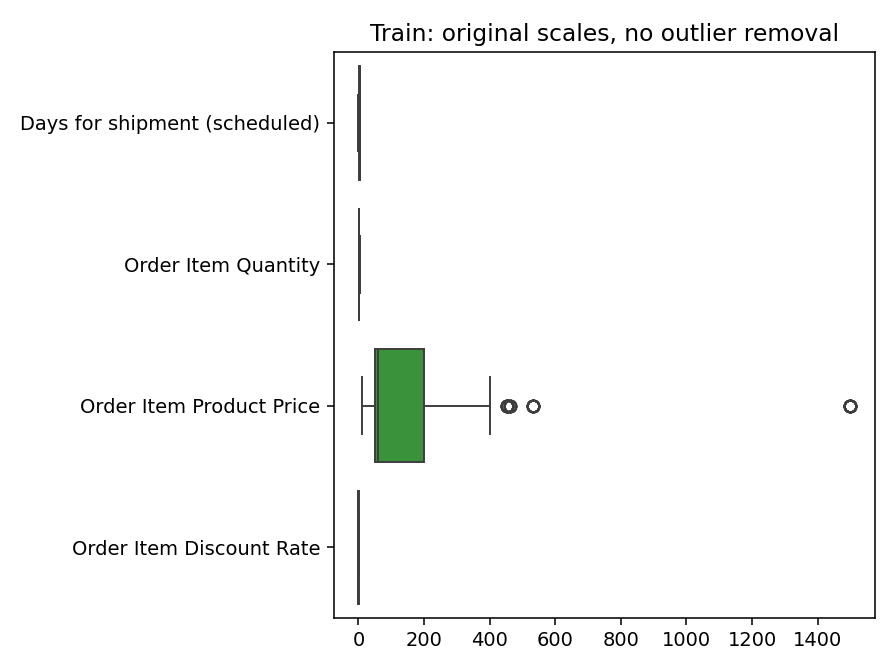
\includegraphics[width=.90\textwidth,height=.42\textheight,keepaspectratio]{../results/figures/04_boxplot.png}\caption{Biểu đồ hộp của các đặc trưng số trên tập huấn luyện.}\label{fig:eda-boxplot}\end{figure}

\begin{figure}[!htbp]\centering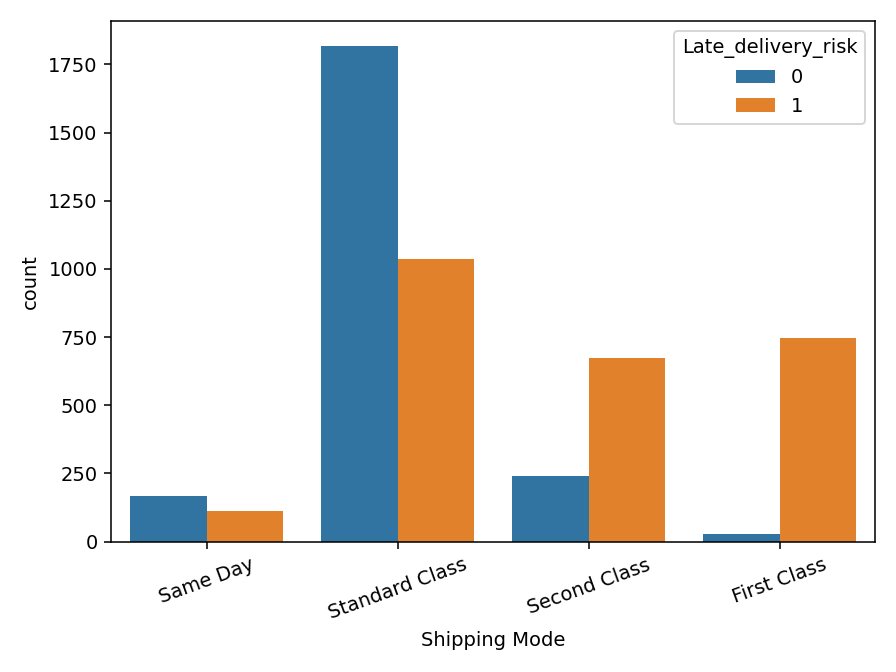
\includegraphics[width=.90\textwidth,height=.42\textheight,keepaspectratio]{../results/figures/05_shipping.png}\caption{Phân bố nhãn theo phương thức giao hàng trên tập huấn luyện.}\label{fig:eda-shipping}\end{figure}

\begin{figure}[!htbp]\centering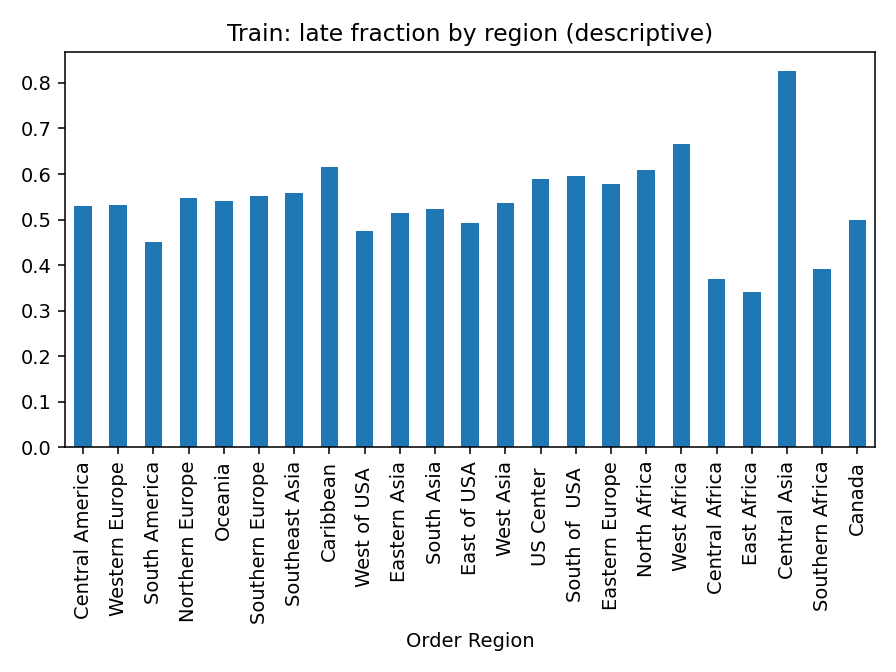
\includegraphics[width=.90\textwidth,height=.42\textheight,keepaspectratio]{../results/figures/06_regions.png}\caption{Phân bố đơn hàng theo vùng trên tập huấn luyện.}\label{fig:eda-regions}\end{figure}

\begin{figure}[!htbp]\centering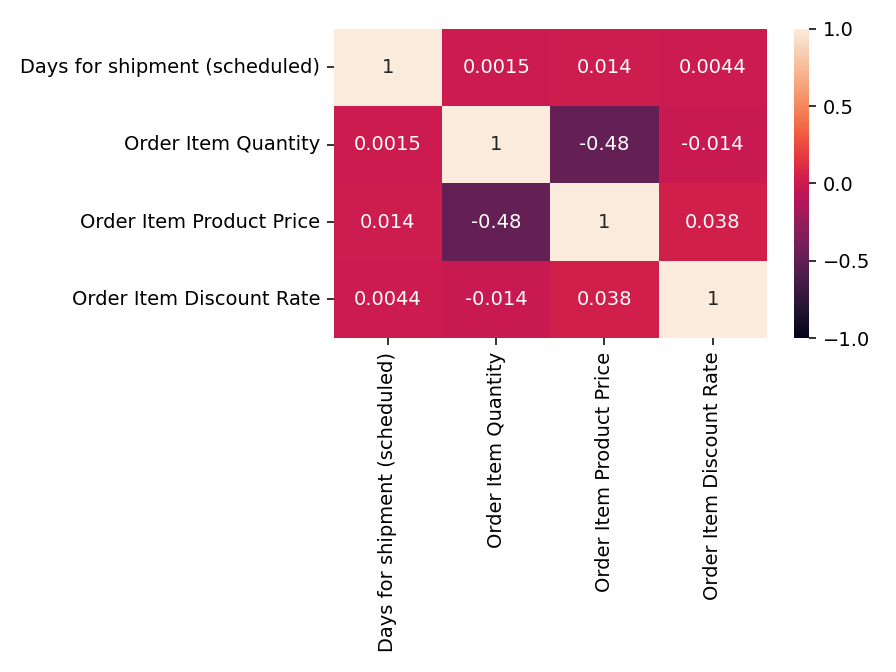
\includegraphics[width=.90\textwidth,height=.42\textheight,keepaspectratio]{../results/figures/07_correlation.png}\caption{Tương quan giữa các đặc trưng số được khảo sát trên tập huấn luyện.}\label{fig:eda-correlation}\end{figure}

\begin{figure}[!htbp]\centering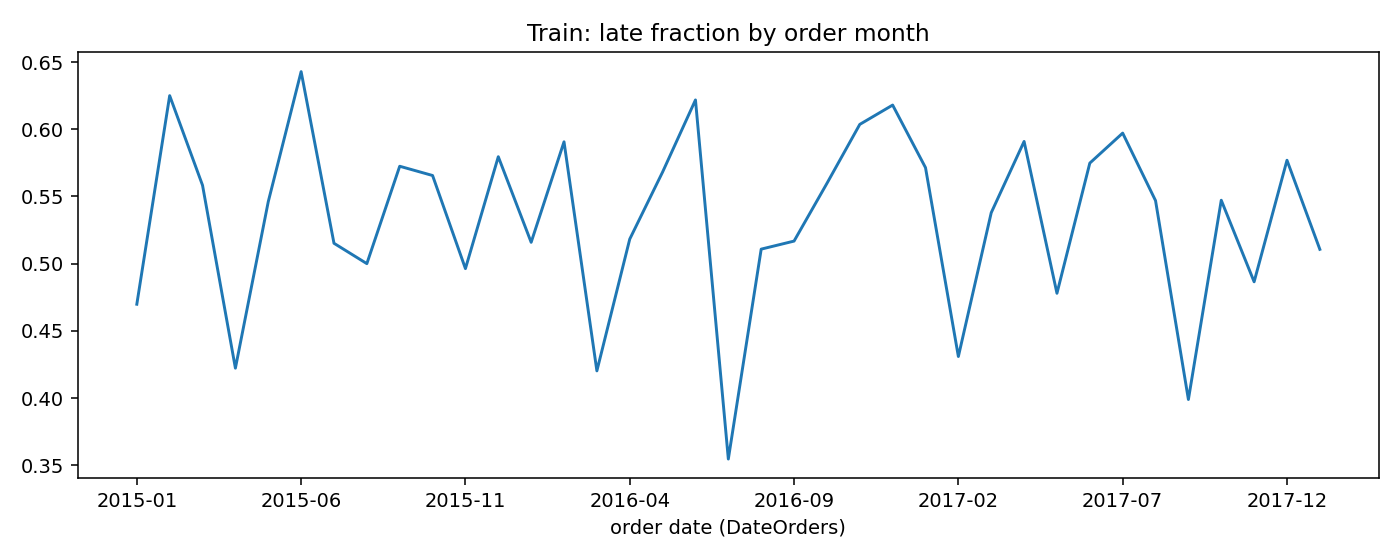
\includegraphics[width=.90\textwidth,height=.42\textheight,keepaspectratio]{../results/figures/08_month.png}\caption{Tỷ lệ giao trễ theo tháng tạo đơn trên tập huấn luyện.}\label{fig:eda-month}\end{figure}